\documentclass[12pt,AutoFakeBold]{article} 

\usepackage[数字信号处理]{XDULabreport}  % 载入 XDULabreport 模板文件,[]中填写科目名称,科目名称,默认为电子线路实验(I)
\problem{信号的频谱分析}  % 请在此处填写问题内容
\labdate{2021年11月10日} % 实验日期
% 其他参数在宏包中进行更改,其中学院,班级,姓名,学号均在sty宏包内进行更改
% \usepackage{fourier}  % 这是 fourier 字体,更柔和 

\newfontfamily\digi{DigifaceWide Regular} % 将数码管字体引入

%% 如果你需要中文的一级标题编号,如“一、”、“二、”等,请把下面两行取消注释
% \RequirePackage{zhnumber} % change section number to chinese
% \titleformat{\section}{\Large\bfseries\rmfamily}{\zhnum{section}、}{0em}{}

% 文档开始
        
\begin{document}

\maketitle
\setcounter{tocdepth}{2}
\tableofcontents  % 生成目录

% 正文标题
\makeatletter
\begin{center}
    \LARGE \textbf{\textsf{\@problem}}
\end{center}
\makeatother

\section{实验目的}

设计计算机程序,产生序列并计算序列的 FFT 和 IFFT,绘制其幅频特性和相频特性曲线;模拟产生离散系统的输入序列和单位脉冲响应,利用 FFT 和 IFFT 算法计算系统的输出响应,分析 FFT 的计算长度对系统输出响应的影响;模拟产生连续时间信号,选取适当的采样频率对其采样,并用 FFT 算法计算其频谱,分析信号的观测时间长度、FFT的计算长度对信号频谱计算结果的影响。

\section{实验原理}

\subsection{离散傅里叶变换(DFT)}

\subsubsection{离散傅里叶变换的定义}

设 $x(n)$ 是长度为 $N$ 的有限长序列,$\tilde{x}(n)$ 是 $x(n)$ 的周期延拓,可写成
%
\begin{equation*}
\tilde{x}(n)=\sum_{l=-\infty}^\infty x(n+lN)
\end{equation*}
% 
显然,$x(n)$ 是 $\tilde{x}(n)$ 的主值序列,表示为
%
\begin{equation*}
x(n)=\tilde{x}(n)R_N(n)
\end{equation*}
%
式中,$R_N(n)$ 为矩形序列,即
%
\begin{equation*}
R_N(n)=\begin{cases}
1,& 0\le n\le N-1 \\
0,& others
\end{cases}
\end{equation*}
%
为方便起见,引入符号 $((n))_N$ 表示 $n$ 对 $N$ 求余数。令 $n=n_1+n_2N$,其中,$0\le n_1\le N-1$,则 $n_1$ 为 $n$ 对 $N$ 的余数,记作 $((n))_N$。$x(n)$ 又可表示为
%
\begin{equation*}
\tilde{x}(n)=x((n))_N
\end{equation*}
%
有限长序列 $X(k)$ 为 $\tilde{X}(k)$ 的主值序列,$\tilde{X}$ 是 $X(k)$ 的周期拓扑,即
%
\begin{equation*}
\tilde{X}(k)=X((k))_N,\quad X(k)=\tilde{X}(k)R_N(k)
\end{equation*}
%
周期序列 $\tilde{x}(n)$ 的 DFS 序列变换对为
%
\begin{equation*}
\tilde{X}(k)=\sum_{n=0}^{N-1}\tilde{x}(n)W_N^{kn},\quad \tilde{x}(n)=\frac{1}{N}\sum_{k=0}^{N-1}\tilde{X}(k)W_N^{-kn}
\end{equation*}
%
它们的求和只限于主值区间,因而这种变换关系也适用于主值序列 $x(n)$ 和 $X(k)$,于是得到长度为 $N$ 的有限长序列 $x(n)$ 的离散傅里叶变换的定义式
%
\begin{align*}
X(k) &= \mathrm{DFT}[x(n)]=\sum_{n=0}^{N-1}W_N^{kn},\quad 0\le k\le N-1 \\
x(n) &= \mathrm{IDFT}[X(k)]=\frac{1}{N}\sum_{k=0}^{N-1}X(k)W_N^{-kn},\quad 0\le n\le N-1
\end{align*}
%
上面两式分别是离散傅里叶变换和离散傅里叶逆变换。$x(n)$ 与 $X(k)$ 构成了离散傅里叶变换对。已知 $x(n)$ 就能够唯一地确定了 $X(k)$,同样,已知 $X(k)$ 就唯一地确定了 $x(n)$。

\subsubsection{离散傅里叶变换的矩阵表示}

设 $\boldsymbol{x}$ 为由 $x(n)(0\le n\le N-1)$ 构成的列向量,$\boldsymbol{X}$ 为由 $X(k)(0\le k\le N-1)$ 构成的列向量,即
%
\begin{equation*}
\boldsymbol{x}=\begin{bmatrix}
x(0) \\
x(1) \\
\vdots \\
x(N-1)
\end{bmatrix}
,\quad
\boldsymbol{X}=\begin{bmatrix}
X(0), \\
X(1), \\
\vdots \\
X(N-1)
\end{bmatrix}
\end{equation*}
%
则有 DFT 矩阵方程
%
\begin{equation*}
\boldsymbol{X}=\boldsymbol{W}_N\boldsymbol{x}
\end{equation*}
%
式中
%
\begin{equation*}
\boldsymbol{W}_N=\begin{bmatrix}
1 & 1 & 1 & \cdots & 1 \\
1 & W_N^1 & W_N^2 & \cdots & W_N^{(N-1)} \\
1 & W_N^2 & W_N^4 & \cdots & W_N^{2(N-1)} \\
\vdots & \vdots & \vdots & & \vdots \\
1 & W_N^{(N-1)} & W_N^{2(N-1)} & \cdots & W_N^{(N-1)(N-1)}
\end{bmatrix}
\end{equation*}
%
为 $N\times N$ 矩阵,其 $(i+1)$ 行 $(j+1)$ 列元素为 $W_N^{ij}(i,j=0,1,\cdots,N-1)$。类似地,IDFT 的矩阵方程为
%
\begin{equation*}
\boldsymbol{x}=(\boldsymbol{W}_N)^{-1}\boldsymbol{X}
\end{equation*}
%
式中
%
\begin{equation*}
\boldsymbol{W}_N^{-1}=\begin{bmatrix}
1 & 1 & 1 & \cdots & 1 \\
1 & W_N^{-1} & W_N^{-2} & \cdots & W_N^{-(N-1)} \\
1 & W_N^{-2} & W_N^{-4} & \cdots & W_N^{-2(N-1)} \\
\vdots & \vdots & \vdots & & \vdots \\
1 & W_N^{-(N-1)} & W_N^{-2(N-1)} & \cdots & W_N^{-(N-1)(N-1)}
\end{bmatrix}
\end{equation*}
%
为 $N\times N$ 矩阵,其 $(i+1)$ 行 $(j+1)$ 列元素为 $W_N^{-ij}(i,j=0,1,\cdots,N-1)$。

\subsubsection{利用 DFT 计算序列的线性卷积}

线性卷积是离散时间信号处理的重要运算,如离散时间系统的时域响应就是通过系统的输入序列与系统的单位脉冲响应的线性卷积而得到的。但在时域中进行线性卷积效率是很低的。由于序列的DFT和IDFT都存在快速算法,因而利用 DFT 来实现序列的线性卷积,可以极大地提高计算线性卷积的效率。

如果 $f(n)=x(n)\otimes y(n)=\displaystyle\sum_{m=0}^{N-1}x(m)y((n-m))_NR_N(n)$ 且
%
\begin{align*}
X(k)&=\mathrm{DFT}[x(n)],\quad 0\le k\le N-1 \\
Y(k)&=\mathrm{DFT}[y(n)],\quad 0\le k\le N-1
\end{align*}
%
则由时域循环卷积定理得
\begin{equation*}
F(k)=X(k)Y(k),\quad 0\le k\le N-1
\end{equation*}
%
从而
\begin{equation*}
f(n)=\mathrm{IDFT}[F(k)],\quad 0\le k\le N-1
\end{equation*}
%
由此可见,序列 $x(n)$ 与 $y(n)$ 的循环卷积既可以在时域直接计算,也可以在频域计算。由于 DFT 和 IDFT 都可以采用快速算法,当 $N$ 很大时,在频域计算的速度要快得多,因而常用 DFT 的快速算法计算序列的循环卷积。

在实际应用中,通常需要计算两个序列的线性卷积,为了提高计算效率,希望采用具有快速算法的 DFT 来实现。然而,DFT 只能计算循环卷积,因此应寻找出两个序列线性卷积与循环卷积之间的关系以及循环卷积与线性卷积相等的条件。

假设 $h(n)$ 和 $x(n)$ 都是有限长序列,长度分别为 $N$ 和 $M$。它们的线性卷积和循环卷积分别表示如下:
%
\begin{align*}
y_l(n) &= h(n) * x(n)=\sum_{m=-\infty}^\infty h(m)x(n-m)=\sum_{m=0}^{L-1}h(m)x(n-m) \\
y_c(n) &= h(n) \oplus x(n)=\sum_{m=0}^{L-1}h(m)x((n-m))_LR_L(n)
\end{align*}
%
式中,$L\ge\max{[N,M]}$,$x((n))_L=\displaystyle\sum_{q=-\infty}^\infty x(n+qL)$,所以
%
\begin{align*}
y_c(n)&=\sum_{m=0}^{L-1}h(m)\sum_{q=-\infty}^\infty x(n-m+qL)R_L(n) \\
&=\sum_{q=-\infty}^\infty\sum_{m=0}^{L-1}h(m)x(n-m+qL)R_L(n)
\end{align*}
%
对照上式可以看出,上式中
%
\begin{equation*}
\sum_{m=0}^{L-1} h(m)x(n-m+qL)=y_l(n+qL)
\end{equation*}
%
因此
\begin{equation*}
y_c(n)=\sum_{q=-\infty}^\infty y_1(n+qL)R_L(n)
\end{equation*}
%
上式说明,$y_c(n)$ 等于 $y_l(n)$ 以 $L$ 为周期的周期延拓序列的主值序列。我们知道,$y_l(n)$ 的长度为 $N+M-1$,因此只有当循环卷积长度 $L\ge N+M-1$ 时,$y_l(n)$ 以 $L$ 为周期进行周期延拓才不会出现混叠现象,此时取其主值序列能够满足 $y_c(n)=y_l(n)$。由此证明了循环卷积等于线性卷积的条件是 $L\ge N+M-1$。


\subsection{快速傅里叶变换(FFT)}

\subsubsection{基 2 时间抽取 FFT 算法}

设序列 $x(n)$ 的长度为 $N(N=2^M, M\in\mathbb{Z})$,按 $n$ 的奇偶性把 $x(n)$ 分解成两个 $\frac{N}{2}$ 点的子序列
%
\begin{align*}
x_1(r) &= x(2r),\quad 0\le r\le N/2-1 \\
x_2(r) &= x(2r+1), \quad 0\le r\le N/2-1
\end{align*}
%
则 $x(n)$ 的 DFT 为
\begin{align*}
X(k) &= \sum_{r=0}^{N/2-1}x(2r)W_N^{2kr}+\sum_{r=0}^{N/2-1}x(2r+1)W_N^{k(2r+1)} \\
     &= \sum_{r=0}^{N/2-1}x_1(r)W_N^{2kr}+W_N^k\sum_{r=0}^{N/2-1}x_2(r)W_N^{2kr}
\end{align*}
%
由旋转因子可约性 $W_N^{2kr}=W_{N/2}^{kr}$ 有
%
\begin{align*}
X(k) &= \sum_{r=0}^{N/2-1}x_1(r)W_{N/2}^{kr}+W_N^k\sum_{r=0}^{N/2-1}x_2(r)W_{N/2}^{kr} \\
     &= X_1(k)+X_2(k),\quad 0\le k\le N/2-1
\end{align*}
%
由于 $X_1(k)$ 和 $X_2(k)$ 具有隐含周期性,周期为 $N/2$,并且旋转因子存在对称性 $W_N^{k+N/2}=-W_N^k$,那么
%
\begin{align*}
X(k) &= X_1(k)+W_N^kX_2(k),\quad 0\le k\le N/2-1 \\
X(k+N/2) &= X_1(k)-W_N^kX_2(k),\quad 0\le k\le N/2-1 
\end{align*}
%
这样就将 $N$ 点 DFT 分解为两个 $N/2$ 点 DFT 和以上两式的运算。
 
\subsubsection{基 2 频域抽取 FFT 算法}

设序列 $x(n)$ 的长度为 $N=2^M$,首先将 $x(n)$ 按 $n$ 的自然顺序前后对半分开,得到两个子序列,其 DFT 可以表示为
%
\begin{align*}
X(k) &= \sum_{n=0}^{N/2-1}x(n)W_N^{kn}+\sum_{n=N/2}^{N-1}x(n)W_N^{kn} \\
     &= \sum_{n=0}^{N/2-1}x(n)W_N^{kn}+\sum_{n=0}^{N/2-1}x\left(n+\frac{N}{2}\right)W_N^{k(n+N/2)} \\
     &= \sum_{n=0}^{N/2-1}\left[x(n)+W_N^{kN/2}x\left(n+\frac{N}{2}\right)\right]W_N^{kn}
\end{align*}
%
式中
%
\begin{equation*}
W_N^{kN/2}=(-1)^k=\begin{cases}
1, & k\ is\ even \\
-1, & k\ is\ odd \\
\end{cases}
\end{equation*}
%
令
%
\begin{align*}
x_1(n) &= x(n)+x\left(n+\frac{N}{2}\right),\quad 0\le n\le N/2-1 \\
x_2(n) &= \left[x(n)-x\left(n+\frac{N}{2}\right)\right]W_N^n,\quad 0\le n\le N/2-1
\end{align*}
%
将 $X(k)$ 分解成偶数组和奇数组,当 $k(k=2r,r=0,1,\cdots,N/2-1)$ 取偶数时
%
\begin{align*}
X(2r) &= \sum_{n=0}^{N/2-1}\left[x(n)+x\left(n+\frac{N}{2}\right)\right]W_N^{2rn} \\
      &= \sum_{n=0}^{N/2-1}x_1(n)W_{N/2}^{rn}
\end{align*}
%
当 $k(k=2r+1,r=0,1,\cdots,N/2-1)$ 取奇数时
%
\begin{align*}
X(2r+1) &= \sum_{n=0}^{N/2-1}\left[x(n)-x\left(n+\frac{N}{2}\right)\right]W_N^{(2r+1)N} \\
        &= \sum_{n=0}^{N/2-1}x_2(n)W_{N/2}^{rn}
\end{align*}
%

\section{实验过程}

\subsection{序列的 FFT 和 IFFT} \label{sec:p1}

设置长度为 16 的序列 $x(n)=[0,1,\cdots,15]$,采用 Python 实现基 2 时间抽取 FFT 算法,序列的 FFT 幅频特性和相频曲线如图 \ref{fig:FFT1} 所示,IFFT 幅频特性和相频曲线如图 \ref{fig:IFFT1} 所示。

\begin{figure}[hbtp]
	\centering
	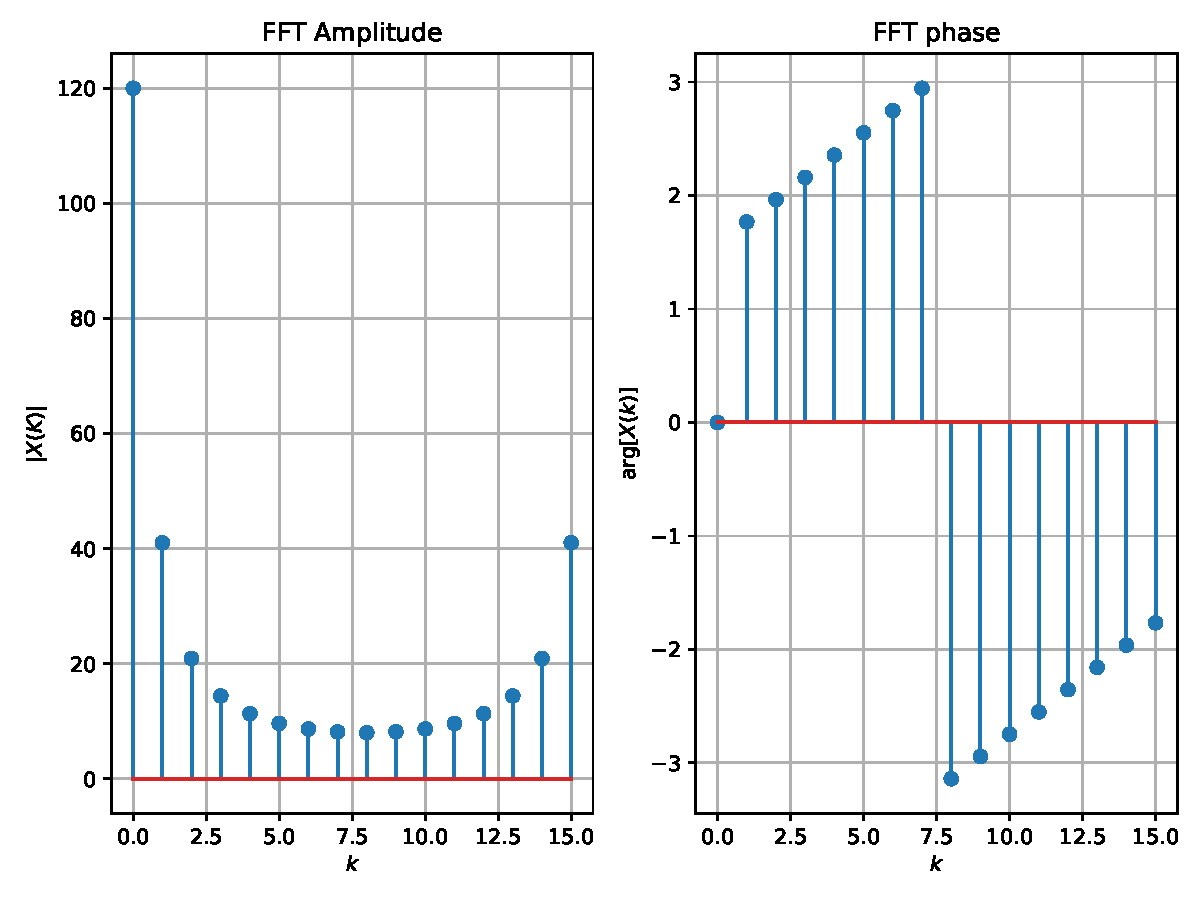
\includegraphics[width=16cm]{FFT1.pdf}
	\caption{序列的 FFT 幅频特性和相频特性曲线}\label{fig:FFT1}
\end{figure}

\begin{figure}[hbtp]
	\centering
	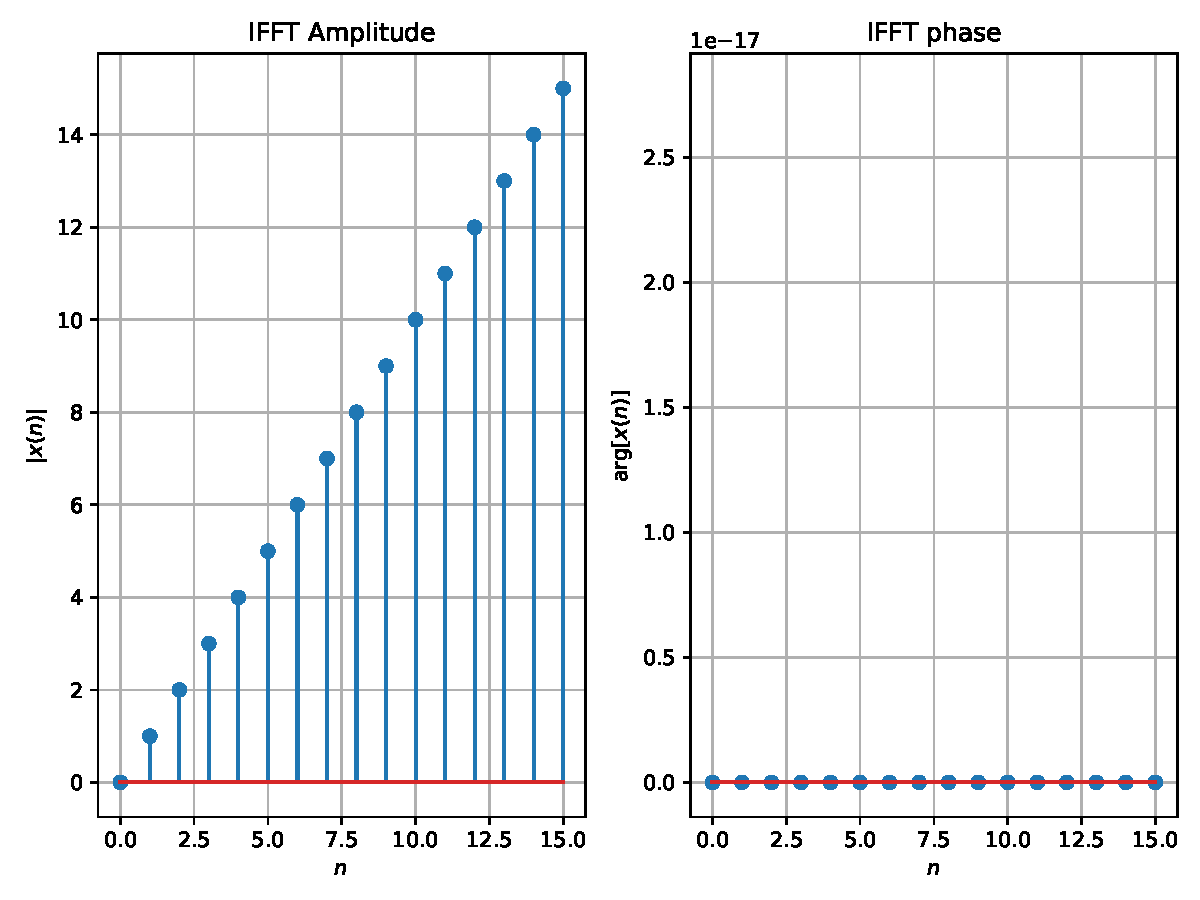
\includegraphics[width=16cm]{IFFT1.pdf}
	\caption{IFFT 幅频特性和相频特性曲线}\label{fig:IFFT1}
\end{figure}

\begin{lstlisting}[language=Python]
#计算FFT和IFFT
import numpy as np
import matplotlib.pyplot as plt

def fft(x):  #基2FFT算法
    x = np.asarray(x, dtype=complex)
    N = x.shape[0]
    if N % 2 > 0:
        raise ValueError("must be a power of 2") # 不符合要求报错
    elif N <= 2:   # 这种情况下直接返回DFT
        n = np.arange(N)
        k = n.reshape((N, 1))
        M = np.exp(-2j * np.pi * n *k/ N)
        return np.dot(M, x)
    else:
        X_even = fft(x[::2])  # 偶数组
        X_odd = fft(x[1::2])  # 奇数组
        terms = np.exp(-2j * np.pi * np.arange(N) / N)
        return np.concatenate([X_even + terms[:int(N/2)] * X_odd,
                               X_even + terms[int(N/2):] * X_odd])

def ifft(x): #直接使用FFT子程序运算ifft
    g = fft(np.conj(x))
    x = np.asarray(x, dtype=complex)
    N = x.shape[0]
    return np.conj(g) / N

k = np.arange(0, 16, 1)
x = k

X = fft(x)
xi = np.fft.ifft(X)  #ifft序列
for i in range(8):
    if np.imag(xi[i]) < 0.001:
        xi = np.real(xi)

#绘制幅频相频图像
plt.figure(figsize=(8, 6), dpi=80)
plt.subplot(121)
plt.stem(k, np.abs(X), use_line_collection=True)
plt.grid()
plt.xlabel('$k$')
plt.ylabel('$|X(K)|$')
plt.title('FFT Amplitude')

plt.subplot(122)
plt.stem(k, np.angle(X), use_line_collection=True)
plt.grid()
plt.xlabel('$k$')
plt.ylabel('$\mathrm{arg}[X(k)]$')
plt.title('FFT phase')
plt.tight_layout()
plt.show()

plt.figure(figsize=(8, 6), dpi=80)
plt.subplot(121)
plt.stem(k, np.abs(xi), use_line_collection=True)
plt.grid()
plt.xlabel('$n$')
plt.ylabel('$|x(n)|$')
plt.title('IFFT Amplitude')

plt.subplot(122)
plt.stem(k, np.angle(xi), use_line_collection=True)
plt.grid()
plt.xlabel('$n$')
plt.ylabel('$\mathrm{arg}[x(n)]$')
plt.title('IFFT phase')
plt.tight_layout()
plt.show()
\end{lstlisting}

\subsection{利用 FFT 和 IFFT 计算系统的输出} \label{sec:p2}

建立系统的差分方程如下
%
\begin{equation*}
y(n)-y(n-1)=x(n)+2x(n-1)
\end{equation*}
%
由系统的差分方程得到系统函数为
%
\begin{equation*}
H(z)=\frac{z+2}{z-1}=1+\frac{3z^{-1}}{1-z^{-1}}
\end{equation*}
%
系统的单位脉冲响应为
%
\begin{equation*}
h(n)=\delta(n)+3u(n-1)
\end{equation*}
%
取其前 10 项参与实验,即 $h(n)=[1,3,3,3,3,3,3,3,3,3]$,其长度为 $N=10$,同时假设输入序列为 $x(n)=[4,3,2,1]$,其长度为 $M=4$,分别取 FFT 的长度为 $L1=8$ 和 $L2=16$ 参与实验,其实验得到的快速线性卷积分别如图 \ref{fig:p11} 所示和如图 \ref{fig:p12} 所示。循环卷积如图 \ref{fig:p2} 所示。实验结果表明,只有当 $L\ge N+M-1$ 时不会出现混叠现象,此时循环卷积等于线性卷积。

\begin{figure}[htbp]
	\centering
	\begin{minipage}[t]{0.48\textwidth}
		\centering
		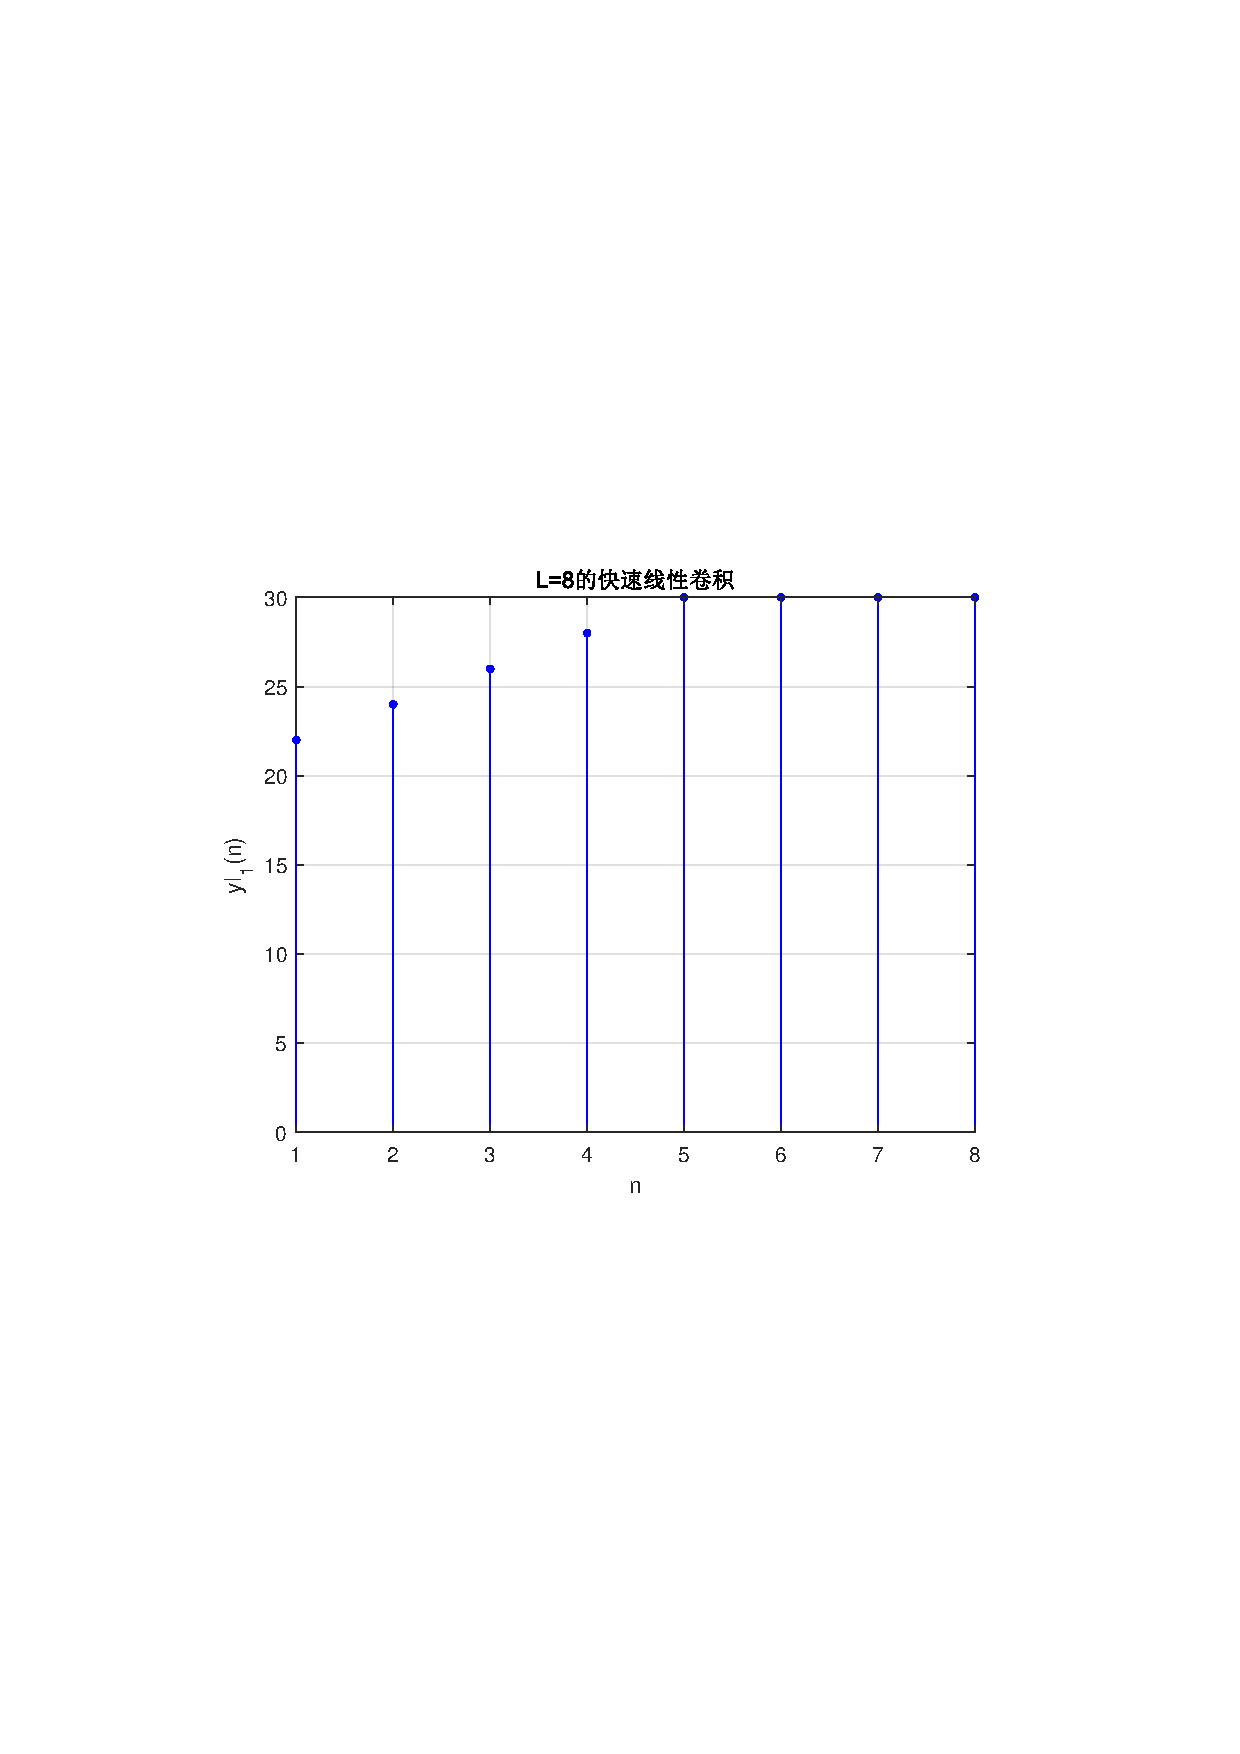
\includegraphics[width=6cm]{figure/p11.pdf}
		\caption{L=8 时的快速线性卷积} \label{fig:p11}
	\end{minipage}
	\begin{minipage}[t]{0.48\textwidth}
		\centering
		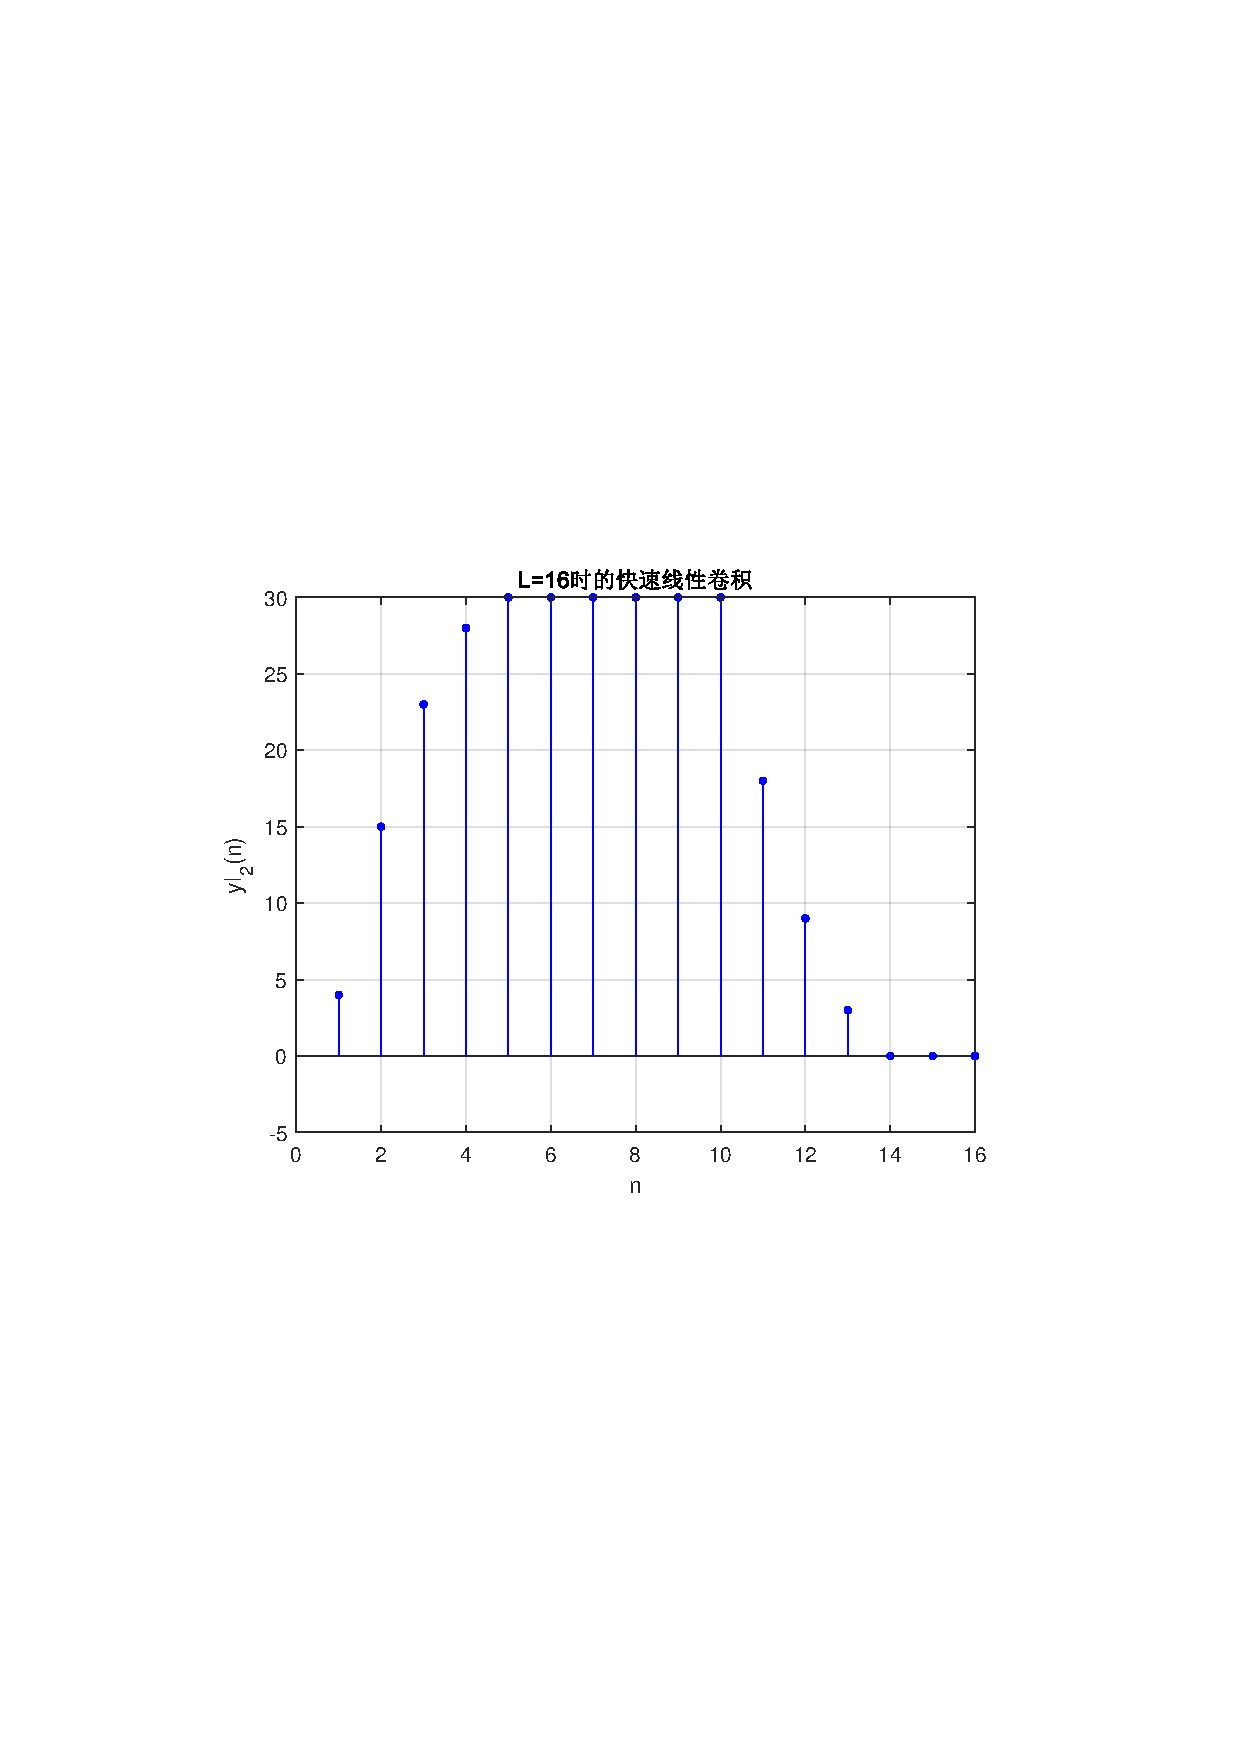
\includegraphics[width=6cm]{figure/p12.pdf}
		\caption{L=16 时的快速线性卷积} \label{fig:p12}
	\end{minipage}
\end{figure}

\begin{figure}[hbtp]
	\centering
	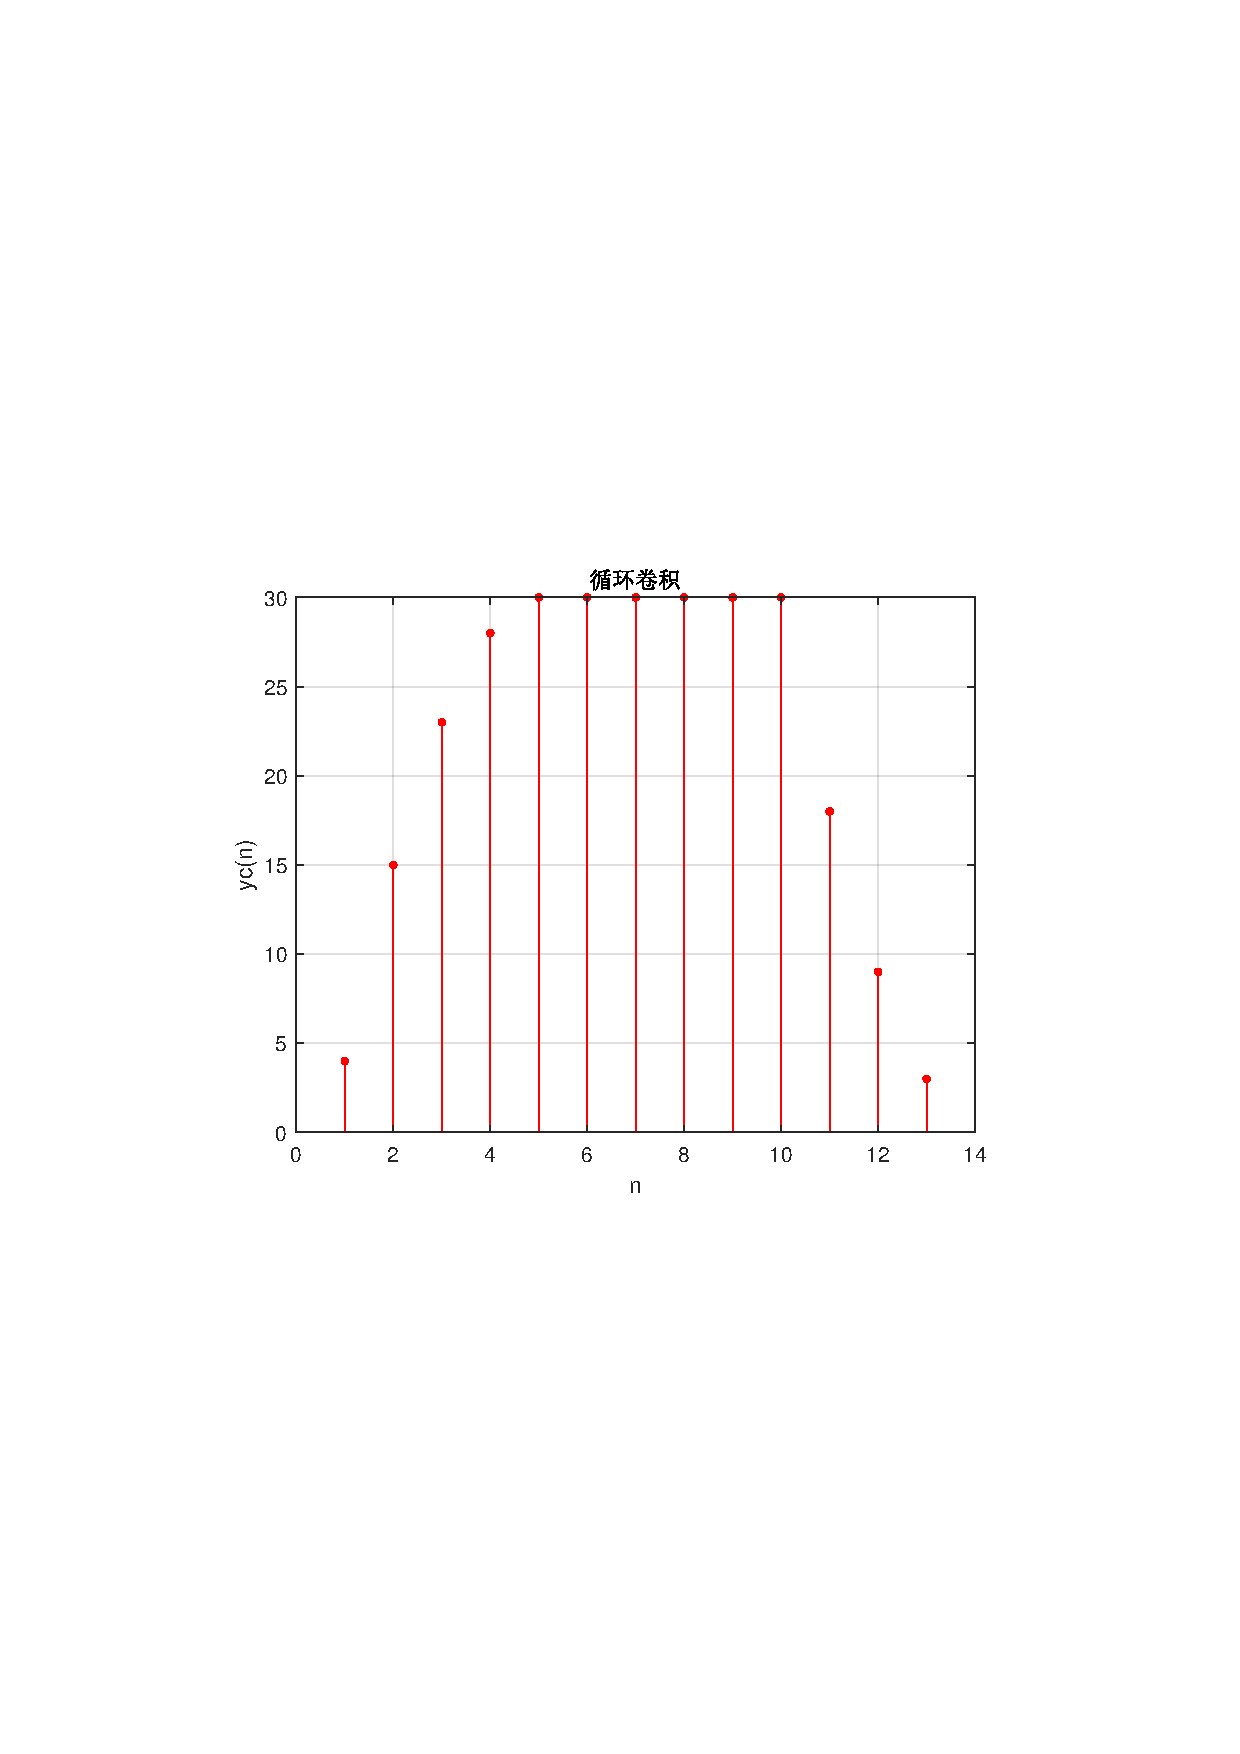
\includegraphics[width=16cm]{p2.pdf}
	\caption{循环卷积}\label{fig:p2}
\end{figure}

\begin{lstlisting}[language=Matlab]
b = [1, 2];
a = [1, -1]; %差分方程的系数
x = [4, 3, 2, 1]'; %输入序列

[h, t] = impz(b, a, 10); %单位脉冲响应

%长度为8
L1 = 8;
X = fft(x, L1);
H = fft(h, L1);
Y = X.*H; %频域相乘
yl1=ifft(Y,L1);

figure(1);
stem(yl1, 'b', 'filled', 'MarkerSize', 3); grid on;
xlabel('n');
ylabel('yl_1(n)');
title('L=8的快速线性卷积')

%长度为16
L2 = 16;
X = fft(x, L2);
H = fft(h, L2);
Y = X.*H; %频域相乘
yl2=ifft(Y,L2);

figure(2);
stem(yl2, 'b', 'filled', 'MarkerSize', 3); grid on;
xlabel('n');
ylabel('yl_2(n)');
title('L=16时的快速线性卷积')

%时域卷积的结果
yc = conv(x, h);

figure(3);
stem(yc, 'r', 'filled', 'MarkerSize', 3); grid on;
xlabel('n');
ylabel('yc(n)');
title('循环卷积')
\end{lstlisting}

\subsection{利用 FFT 分析采样信号} \label{sec:p3}

假设模拟信号 $x_a(t)=2\cos(t)+\sin(2t)$,最高信号频率为 $\frac{1}{\pi}$,采样时间间隔 $T$ 应满足 $T=\frac{1}{f_s}\le\frac{1}{2f_c}=\frac{\pi}{2}$,在 $[0,4\pi)$ 以采样周期 $T=\frac{\pi}{8}$ 对其进行采样得到的长度为 32 的序列为
%
\begin{equation*}
x(n)=x_a(t)|_{t=nT}=2\cos(\frac{\pi n}{8})+\sin(\frac{\pi n}{4})
\end{equation*}
%
采样过程如图 \ref{fig:p31} 所示。

\begin{figure}[hbtp]
	\centering
	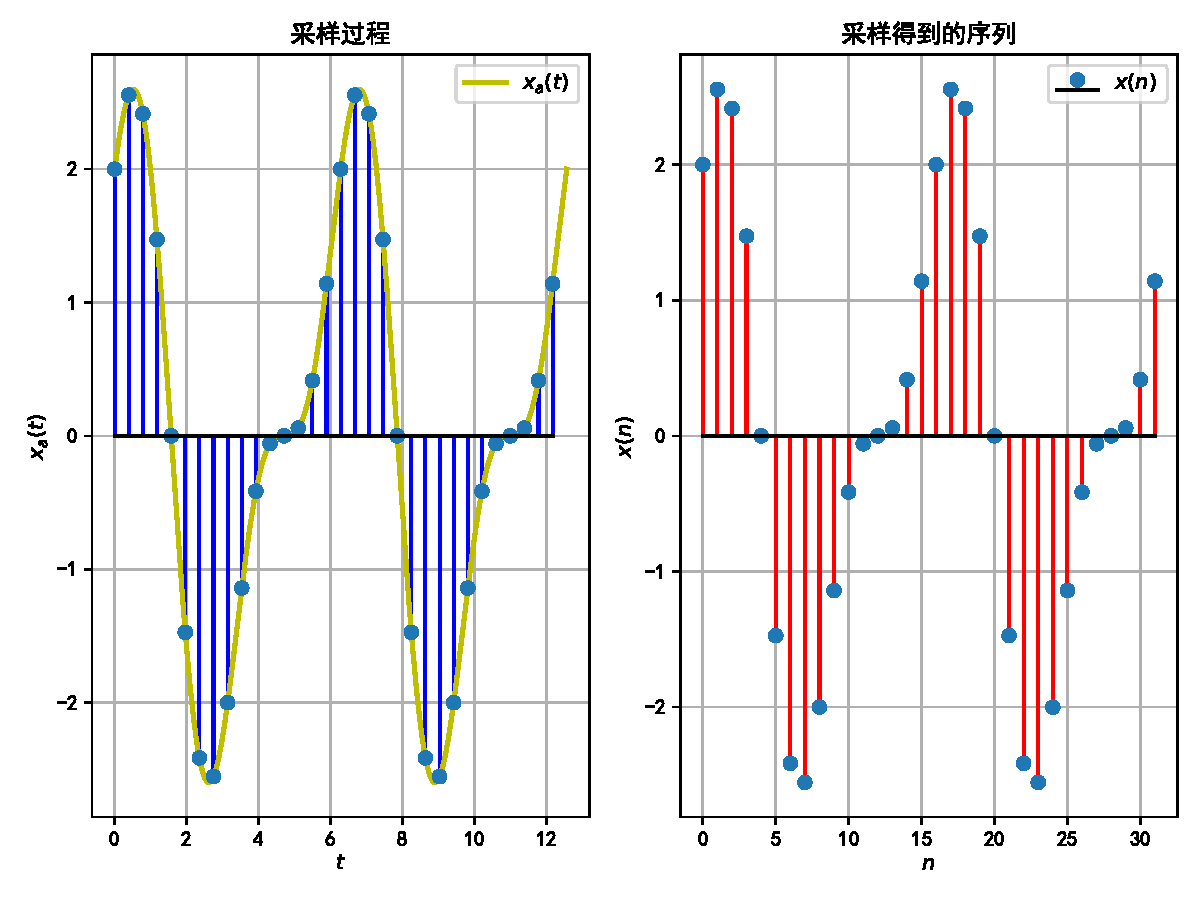
\includegraphics[width=16cm]{p31.pdf}
	\caption{采样过程和得到序列} \label{fig:p31}
\end{figure}

递归递归调用实现的 FFT 算法并不是最优的,可以矢量化将算法变为并行计算,采样序列的 FFT 幅频特性和相频曲线如图 \ref{fig:p32} 所示。同时我们得到的 DTFT 曲线如图 \ref{fig:p33} 所示,可以看出 $X(k)$ 是从 $X(e^{j\omega})$ 以采样角频率 $\Omega=\frac{\pi}{16}$ 采样得到。

信号的持续时间 $T_p$ 应满足频率分辨率 $\Delta f$ 的要求,即
%
\begin{equation*}
T_p=NT=\frac{N}{f_s}=\frac{1}{\Delta f}
\end{equation*}
%
频率分辨率 $\Delta f$ 与信号采样的持续时间 $T_p$ 是反比关系,若希望得到较高的频率分辨率,则需要较长的信号采样持续时间。

\begin{figure}[hbtp]
	\centering
	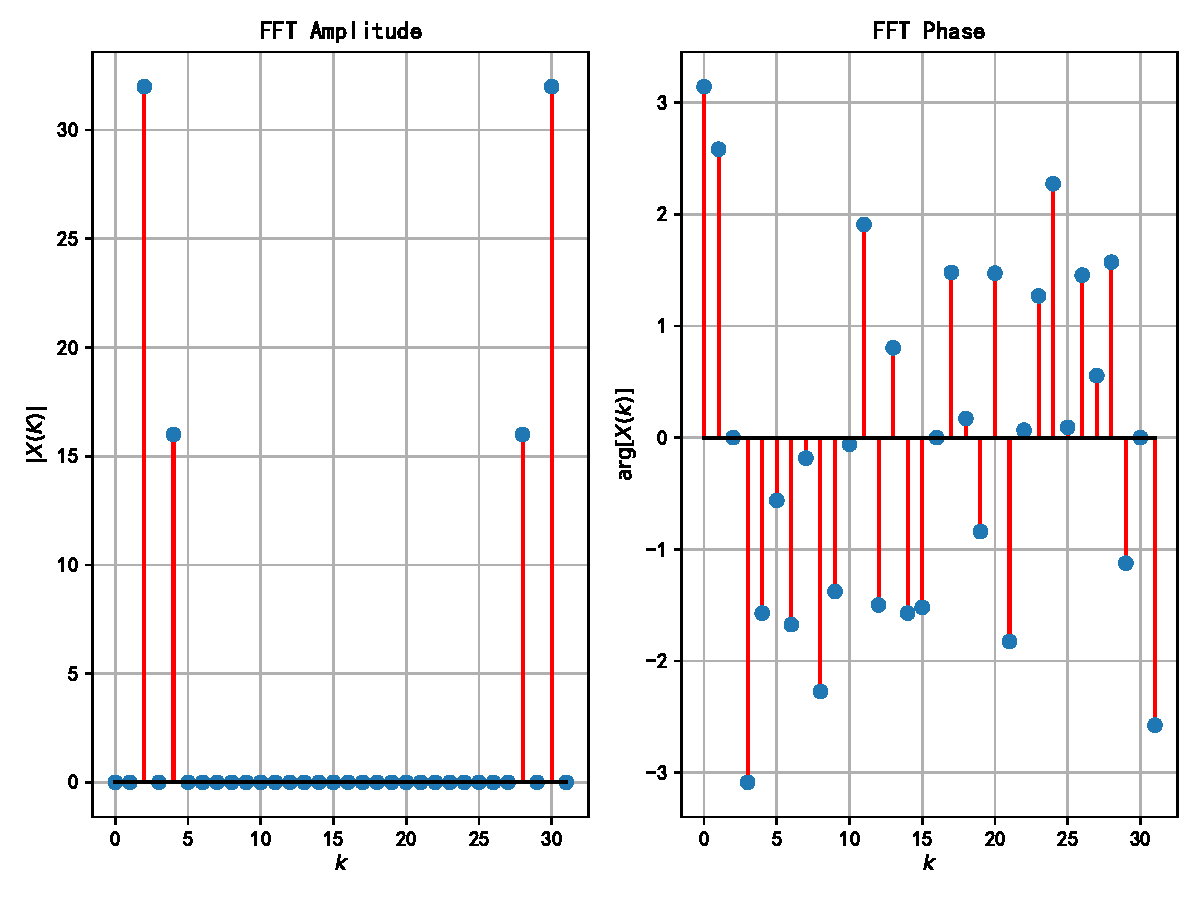
\includegraphics[width=16cm]{p32.pdf}
	\caption{采样序列的 FFT 幅频特性和相频特性曲线} \label{fig:p32}
\end{figure}

\begin{figure}[hbtp]
	\centering
	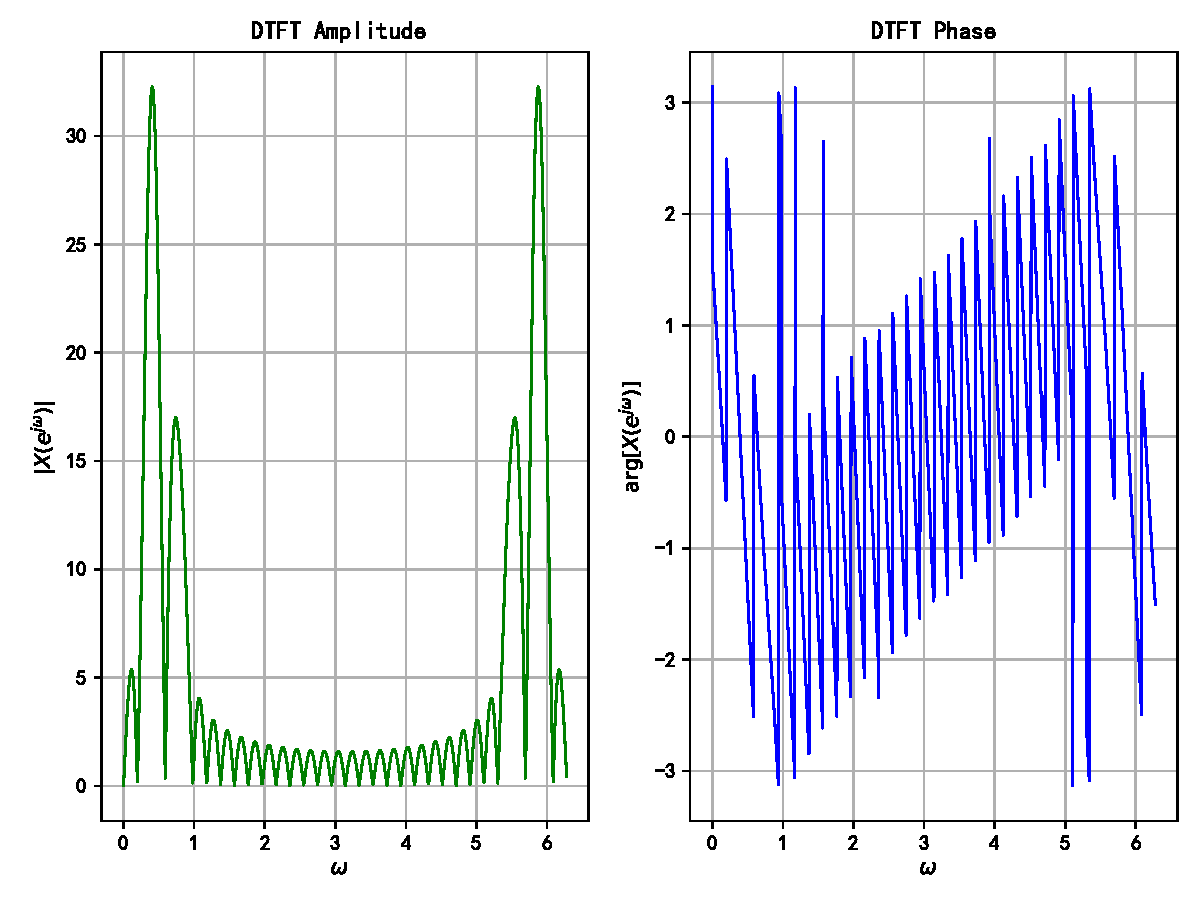
\includegraphics[width=16cm]{p33.pdf}
	\caption{采样序列的 DTFT 幅频特性和相频特性曲线} \label{fig:p33}
\end{figure}

\begin{lstlisting}[language=Python]
import numpy as np
import matplotlib.pyplot as plt

def FFT_Vec(x):
	x = np.asarray(x, dtype=float)
	N = x.shape[0]
	if np.log2(N) % 1 > 0:
		raise ValueError("must be a power of 2")
	N_base = min(N, 2)
	n = np.arange(N_base)
	k = n[:, None]
	X = np.dot(np.exp(-2j * np.pi * n * k / N_base), x.reshape((N_base, -1)))
	while X.shape[0] < N:
		X_even = X[:, :X.shape[1] // 2]
		X_odd = X[:, X.shape[1] // 2:]
		factor = np.exp(-1j * np.pi * np.arange(X.shape[0]) / X.shape[0])[:, None]
		X = np.vstack([X_even + factor * X_odd, X_even - factor * X_odd])
	return X.ravel()

def func(t):
	return 2 * np.cos(t) + np.sin(2 * t)

t = np.linspace(0, 4 * np.pi, 1000)
nt = np.arange(0, 4 * np.pi, np.pi / 8)

plt.rcParams['font.sans-serif'] = ['SimHei']
plt.rcParams['axes.unicode_minus'] = False

plt.figure(figsize=(8, 6), dpi=80)
plt.subplot(121)
plt.plot(t, func(t), 'y', linewidth=2.0, label=r'$x_a(t)$')
plt.stem(nt, func(nt), linefmt='b', basefmt='k-', markerfmt='C0o')
plt.legend(loc='upper right')
plt.grid()
plt.xlabel('$t$')
plt.ylabel('$x_a(t)$')
plt.title('采样过程')

plt.subplot(122)
n = np.arange(0, 32)
xn = func(np.pi * n / 8)
plt.stem(n, xn, linefmt='r', basefmt='k-', markerfmt='C0o', label=r'$x(n)$')
plt.legend(loc='upper right')
plt.grid()
plt.xlabel('$n$')
plt.ylabel('$x(n)$')
plt.title('采样得到的序列')
plt.tight_layout()
plt.show()

n = np.mat(n)
omega = np.arange(0, 2*np.pi , 2*np.pi /1000)
X = xn * np.exp(-1j*n.T*omega)
X = X.T

plt.figure(figsize=(8, 6), dpi=80)
plt.subplot(121)
plt.plot(omega , np.abs(X), 'g', linewidth =1.0)
plt.grid()
plt.xlabel('$\omega$ ')
plt.ylabel('$|X(e^{j\omega })|$')
plt.title('DTFT Amplitude ')

plt.subplot(122)
plt.plot(omega , np.angle(X), 'b', linewidth =1.0)
plt.grid()
plt.xlabel('$\omega$ ')
plt.ylabel('$\mathrm{arg}[X(e^{j\omega })]$')
plt.title('DTFT Phase')
plt.tight_layout()
plt.show()

n = np.arange(0, 32)
X = FFT_Vec(xn)

plt.figure(figsize=(8, 6), dpi=80)
plt.subplot(121)
plt.stem(n, np.abs(X), linefmt='r', basefmt='k-', markerfmt='C0o')
plt.grid()
plt.xlabel('$k$')
plt.ylabel('$|X(K)|$')
plt.title('FFT Amplitude')

plt.subplot(122)
plt.stem(n, np.angle(X), linefmt='r', basefmt='k-', markerfmt='C0o')
plt.grid()
plt.xlabel('$k$')
plt.ylabel('$\mathrm{arg}[X(k)]$')
plt.title('FFT Phase')
plt.tight_layout()
plt.show()
\end{lstlisting}

\section{总结}

\subsection{杨文韬}

主要负责 \LaTeX 排版和 \ref{sec:p3} 部分代码编写。

\begin{itemize}
\item 问题1:如何选择 FFT 的变换区间?

\begin{enumerate}[1.]
\item 对于非周期信号:有频谱分辨率 $\Delta f$,而频谱分辨率和 FFT 的变换区间有关,由于 FFT 能够实现的频率分辨率是 $\frac{2\pi}{N}$,因此有最小的 $N>\frac{2\pi}{\Delta f}$,据此选择 FFT 的变换区间。
\item 对于周期信号,周期信号的频谱是离散谱,只能用整数倍周期的长度作 FFT,得到的离散谱才能代表周期信号的频谱。
\end{enumerate}

\item 问题2:使用 Matplotlib 添加图例时如何解决中文乱码问题?

解决方法:可以通过 \lstinline[language=Python]|plt.rcParams['font.sans-serif'] = ['SimHei']| 和 \lstinline[language=Python]|plt.rcParams['axes.unicode_minus'] = False| 两行代码解决中文乱码问题。
\end{itemize}

\subsection{刘浩}

主要负责 \ref{sec:p1} 部分代码编写。

\begin{itemize}
\item 问题1:如何验证自己的结果是否正确?

解决方法:通过调用 matlab 的 FFT,IFFT 函数或 python numpy 库中的 fft 库的 fft 和 ifft 函数验证相同输入序列的结果的准确性,此外,Python 中提供了 \lstinline[language=Python]|numpy.allclose| 进行序列的比较。
\item 问题2:如何使用 FFT 解决 IFFT 的计算?

解决方法:使用书中直接调用 FFT 子程序法的第一种方法,直接给 FFT 输入 X(k) 的共轭序列,再将返回结果取共轭后除以 N 即可。
\item 问题3:如何利用 python 绘制茎叶图?

解决方法:经查询,我使用了 matplotlib 库中的 stem 函数绘制茎叶图像。
\end{itemize}

\subsection{周泽熙}

主要负责 \ref{sec:p2} 部分代码编写。

\begin{itemize}
\item 问题:如何理解 FFT 中改变 N,系统输出响应的变化?

FFT 是 DFT 的一类算法,本质还是DFT,然而DFT只能计算循环卷积,输出响应序列为单位脉冲响应和输入序列的线性卷积。只有当循环卷积的长度 $\ge$ 输入序列长度 $+$ 单位脉冲响应序列长度 $-1$ 时,循环卷积才会等于线性卷积。所以当 FFT 计算长度 N 较小时,对序列的周期延拓发生了混叠现象,计算出的输出不是真实输出。
\end{itemize}

% % 参考文献,此处以 MLA 引用格式为例

%\begin{thebibliography}{9}
%\end{thebibliography}

% % \includepdf[pages={1,2}]{Memo.pdf} 
% 可以直接导入pdf页面
%\newpage
%\begin{appendices}  % 附录环境
%\section{核心层}\label{subsec:B}
%\end{appendices}

\end{document}  % 结束